\documentclass[11pt]{article}
\usepackage[margin=1in]{geometry}
\usepackage{graphicx}
\usepackage{booktabs}
\usepackage{float}
\usepackage{hyperref}
\usepackage{setspace}
\usepackage[T1]{fontenc}
\usepackage[utf8]{inputenc}
\onehalfspacing

\title{Time-Series-Driven Predictive Maintenance}
\author{Stat 248 Final Project}
\date{\today}

\begin{document}
\maketitle

\begin{abstract}
This project studies predictive maintenance as a time-series forecasting problem with an operational decision layer. A synthetic fleet of degrading machines generates vibration, temperature, and pressure signals over time. The main question is whether richer temporal summaries improve short-horizon failure-risk prediction and, in turn, lower maintenance cost. Results show that nonlinear time-series features improve predictive accuracy over raw-sensor baselines, and a simple risk-threshold policy outperforms reactive and fixed-schedule maintenance. The main lesson is that better temporal representation matters more than a more complicated controller.
\end{abstract}

\section{Introduction}
Predictive maintenance is a natural time-series problem because machine failure is driven by the evolution of degradation rather than by one isolated sensor reading. In this project, the main objective is to determine whether temporal summaries extracted from sensor streams improve near-term failure prediction. A secondary objective is to show that better risk estimates can be converted into better maintenance decisions.

\section{Data-Generating Process}
The project uses a fully synthetic but reproducible fleet simulation. Each machine has a latent health process, a stressed operating regime, and three observed sensors: vibration, temperature, and pressure. Machines fail when latent health falls below a threshold or when a high-hazard event occurs near the end of life. The supervised label at each timestamp is whether failure occurs within the next eight periods.

\begin{table}[H]
\centering
\caption{Summary of the generated dataset across train, validation, and test splits.}
\label{tab:data-summary}
\resizebox{\textwidth}{!}{%
\begin{tabular}{lrrrrrrrrrr}
\toprule
split & n\_rows & n\_machines & mean\_failure\_time & mean\_path\_length & vibration\_min & vibration\_max & temperature\_min & temperature\_max & pressure\_min & pressure\_max \\
\midrule
train & 4726 & 90 & 51.5111 & 52.5111 & 0.2684 & 1.6225 & 57.0486 & 75.6074 & 96.5649 & 106.9888 \\
validation & 1723 & 35 & 48.2286 & 49.2286 & 0.2871 & 1.6209 & 58.5078 & 75.6872 & 96.9107 & 106.9589 \\
test & 1941 & 35 & 54.4571 & 55.4571 & 0.3233 & 1.5428 & 58.0908 & 75.3467 & 96.9284 & 107.4286 \\
\bottomrule
\end{tabular}}
\end{table}

\section{Methods}
Three predictive models are compared. The baseline GLM uses current age and raw sensor values. The advanced GLM adds rolling means, rolling standard deviations, rolling slopes, and Holt level-trend summaries. The nonlinear time-series forest extends this feature set with multi-scale rolling summaries, lags, first and second differences, exponentially weighted moving averages, and stress-contrast variables.

To connect prediction with decision-making, the project compares reactive maintenance, fixed-age replacement, a tuned risk-threshold policy, tabular Q-learning, and a compact DQN extension. The RL methods are included as benchmarks, but the main focus remains on the time-series forecasting layer.

\section{Predictive Results}
\begin{table}[H]
\centering
\caption{Predictive performance on the test fleet.}
\label{tab:risk-metrics}
\resizebox{\textwidth}{!}{%
\begin{tabular}{lrrr}
\toprule
model & auc & brier & log\_loss \\
\midrule
nonlinear\_ts\_forest & 0.8821 & 0.0922 & 0.2972 \\
advanced\_glm & 0.8790 & 0.0935 & 0.2997 \\
baseline\_glm & 0.8732 & 0.0949 & 0.3045 \\
\bottomrule
\end{tabular}}
\end{table}
The best predictive model is \texttt{nonlinear\_ts\_forest}. This supports the claim that explicit temporal representation improves short-horizon failure prediction beyond current sensor levels alone.

\begin{table}[H]
\centering
\caption{Top ten feature importances for the nonlinear time-series forest.}
\label{tab:feature-importance}
\resizebox{\textwidth}{!}{%
\begin{tabular}{lr}
\toprule
feature & importance \\
\midrule
vibration\_mean\_15 & 0.0932 \\
vibration\_mean\_8 & 0.0728 \\
vibration\_ewm\_04 & 0.0627 \\
pressure\_ewm\_04 & 0.0518 \\
holt\_level & 0.0517 \\
pressure\_mean\_15 & 0.0480 \\
pressure\_mean\_8 & 0.0468 \\
health\_proxy & 0.0412 \\
pressure\_mean\_3 & 0.0392 \\
vibration & 0.0329 \\
\bottomrule
\end{tabular}}
\end{table}

\begin{figure}[H]
\centering
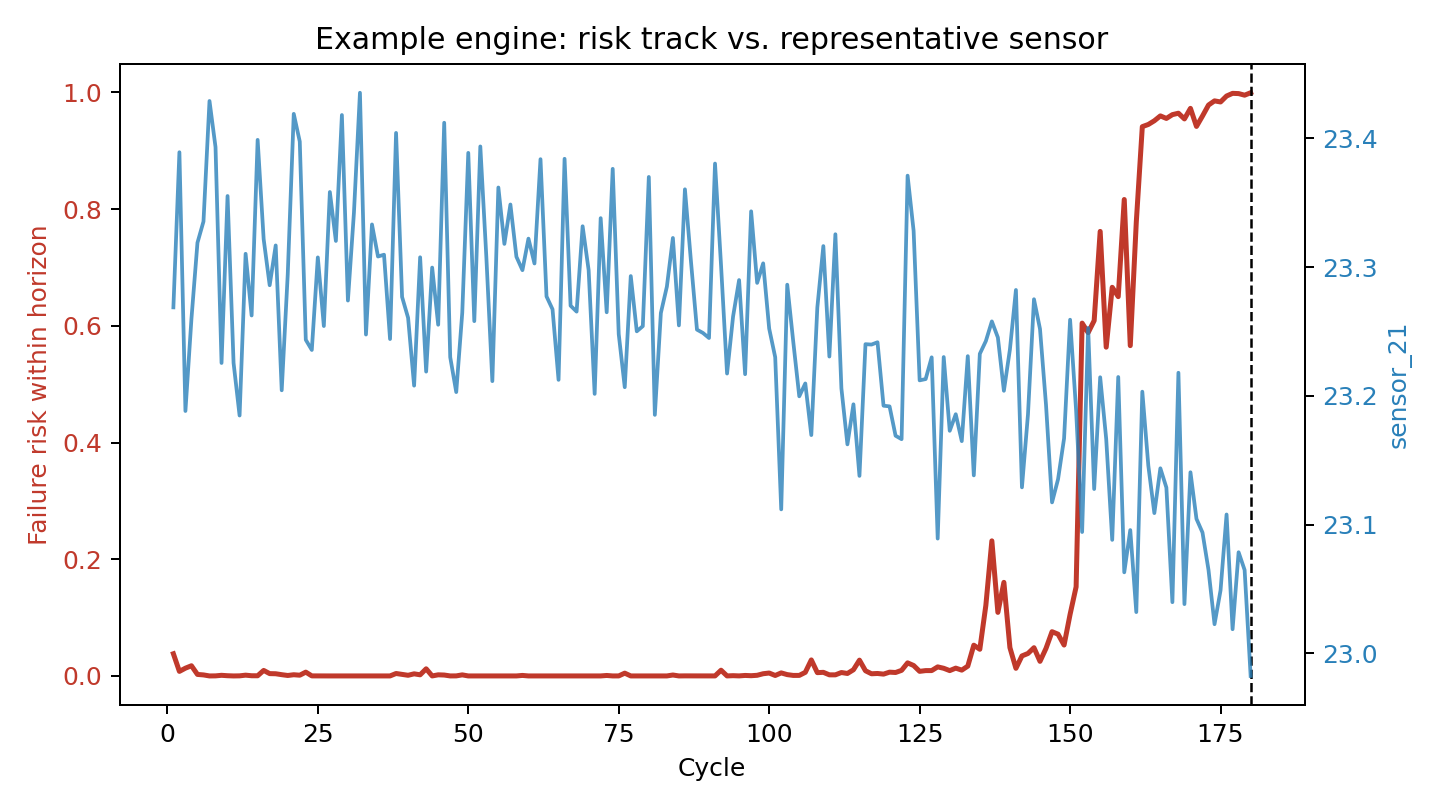
\includegraphics[width=0.82\textwidth]{../outputs/example_risk_path.png}
\caption{Predicted short-horizon failure risk for one example machine, shown alongside a representative sensor path.}
\label{fig:risk-path}
\end{figure}

\begin{figure}[H]
\centering
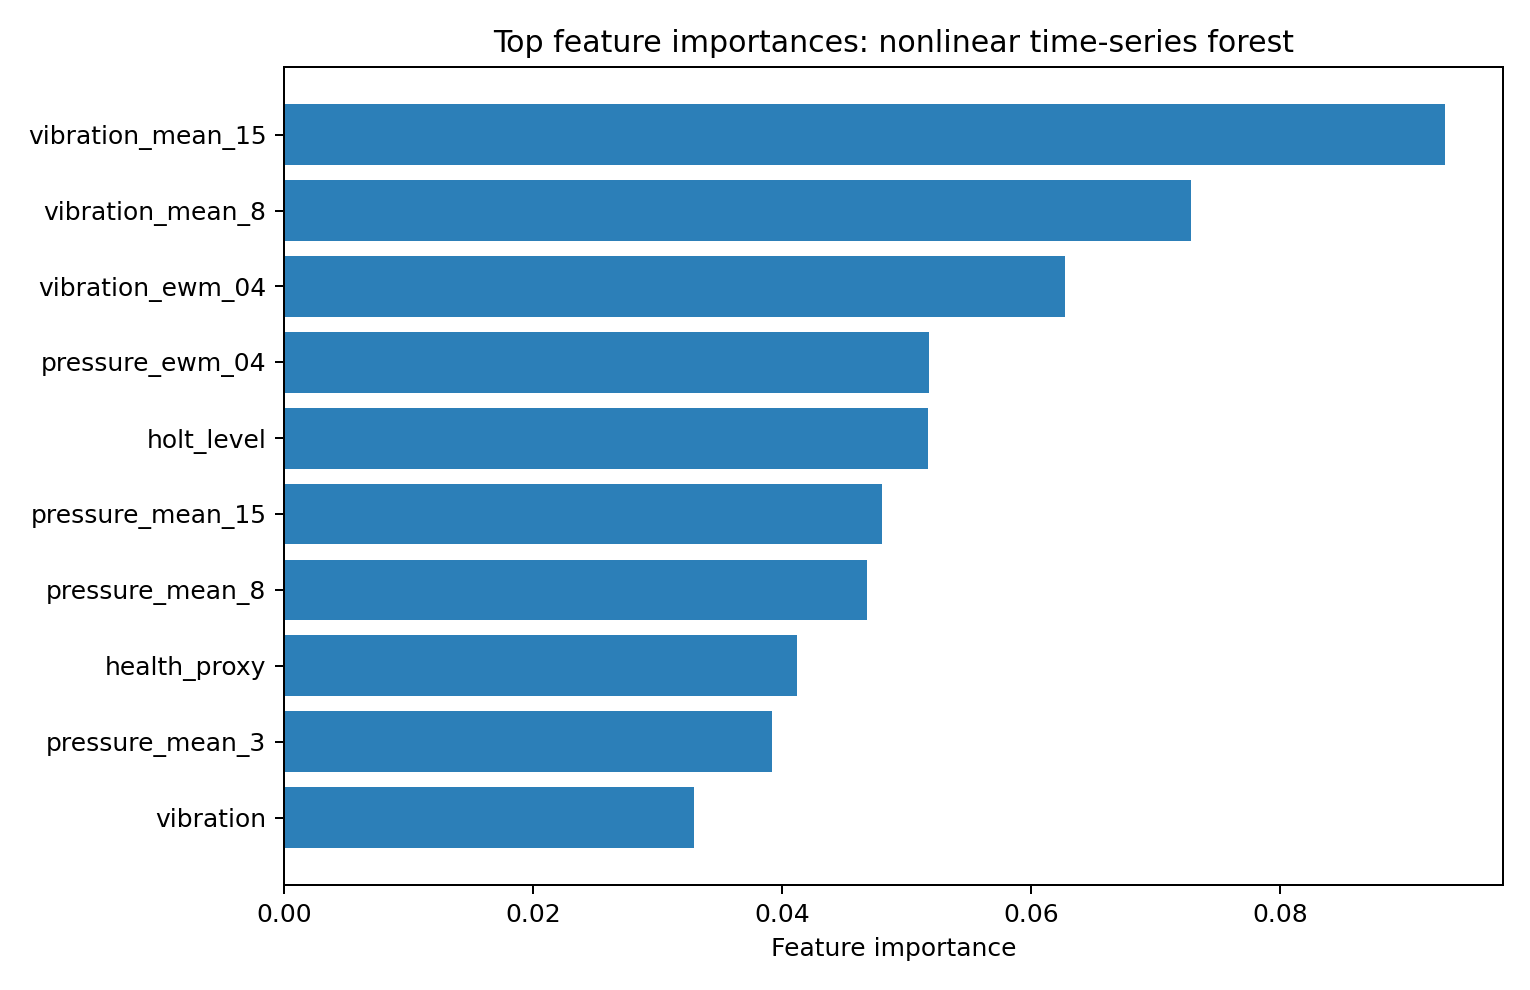
\includegraphics[width=0.72\textwidth]{../outputs/feature_importance_top10.png}
\caption{Top feature importances for the nonlinear time-series forest.}
\label{fig:feature-importance}
\end{figure}

\section{Diagnostics}
To validate the time-series workflow, the project includes augmented Dickey-Fuller checks on first-differenced sensor series, calibration summaries for predicted probabilities, and residual dependence diagnostics.

\begin{table}[H]
\centering
\caption{ADF diagnostics on first-differenced sensor series.}
\label{tab:stationarity}
\resizebox{\textwidth}{!}{%
\begin{tabular}{lrrr}
\toprule
series & adf\_stat & p\_value & crit\_5pct \\
\midrule
vibration\_first\_difference & -19.0789 & 0.0000 & -2.8622 \\
temperature\_first\_difference & -18.2645 & 0.0000 & -2.8622 \\
pressure\_first\_difference & -22.7867 & 0.0000 & -2.8622 \\
\bottomrule
\end{tabular}}
\end{table}

\begin{figure}[H]
\centering
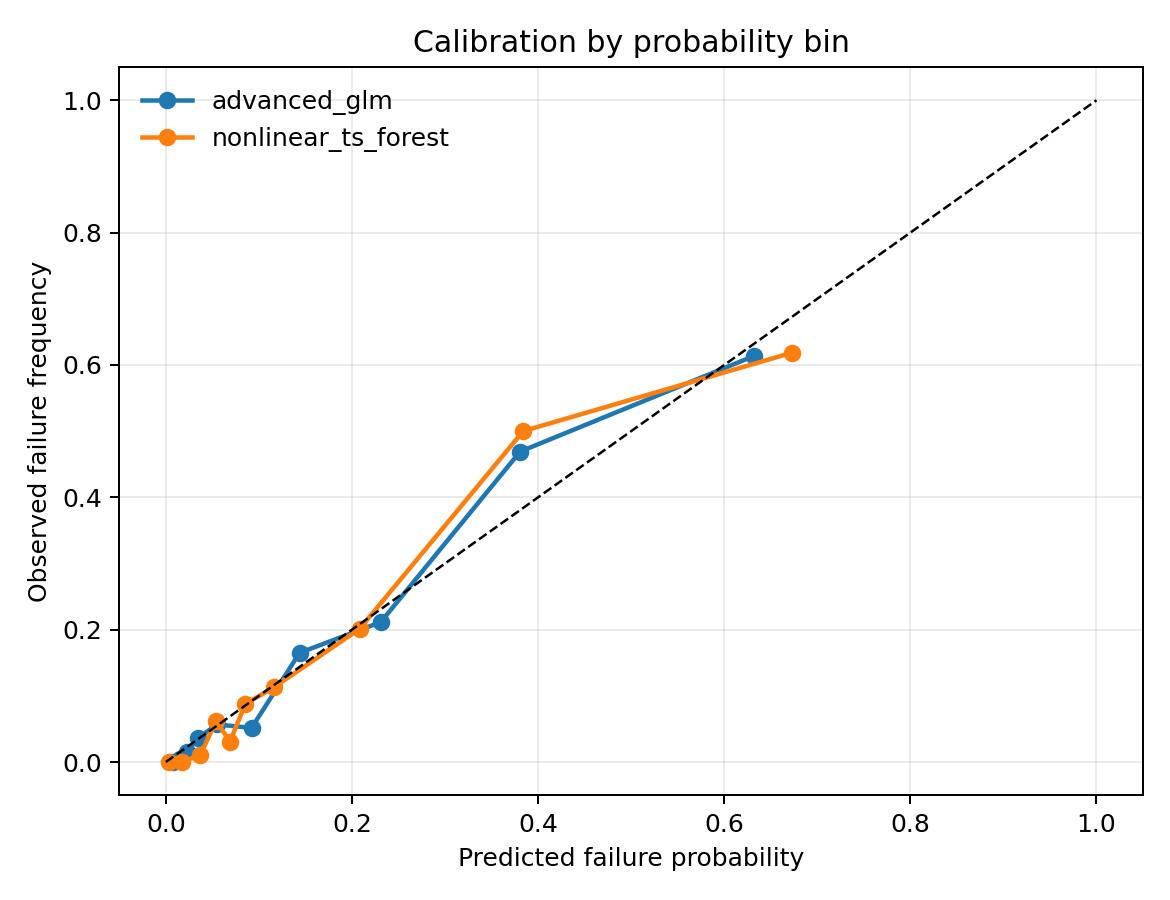
\includegraphics[width=0.48\textwidth]{../outputs/calibration_curve.png}
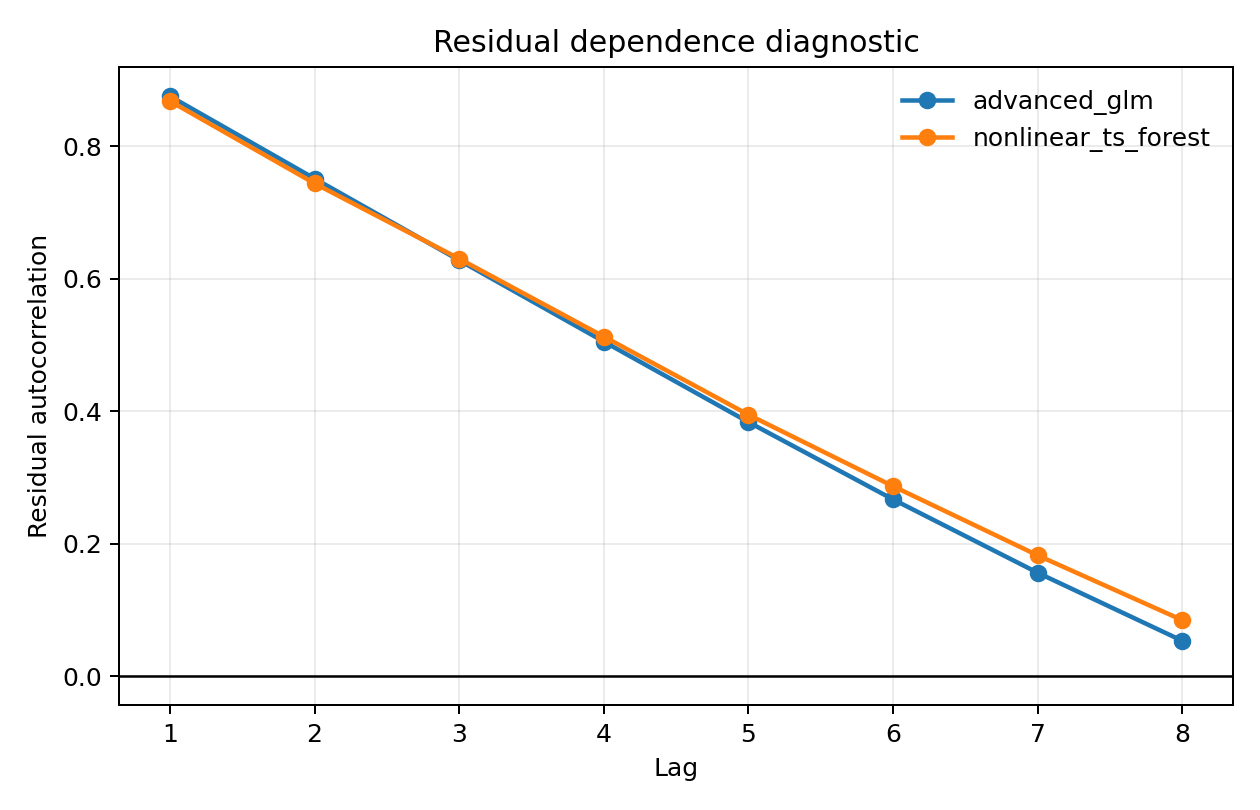
\includegraphics[width=0.48\textwidth]{../outputs/residual_acf.png}
\caption{Calibration and residual dependence diagnostics for the strongest predictive models.}
\label{fig:diagnostics}
\end{figure}

\section{Maintenance Policy Comparison}
Policies are evaluated in a continuing-operation environment in which each replacement starts a fresh machine. Preventive replacement costs 18 units, while failure-driven replacement costs 95 units.

\begin{table}[H]
\centering
\caption{Average cost and event counts by maintenance policy.}
\label{tab:policy-results}
\resizebox{\textwidth}{!}{%
\begin{tabular}{lrrrr}
\toprule
policy & avg\_reward & avg\_cost & avg\_replacements & avg\_failures \\
\midrule
risk\_threshold\_0.25 & -77.6429 & 77.6429 & 2.7857 & 0.3571 \\
q\_learning & -100.4286 & 100.4286 & 4.3571 & 0.2857 \\
age\_threshold\_75 & -200.6429 & 200.6429 & 2.2857 & 2.0714 \\
reactive & -203.5714 & 203.5714 & 2.1429 & 2.1429 \\
dqn & -223.9286 & 223.9286 & 2.3571 & 2.3571 \\
\bottomrule
\end{tabular}}
\end{table}

The tuned risk-threshold rule uses a threshold of 0.25. It achieves the lowest average cost in this experiment, which reinforces the main story of the project: once the risk estimate is informative, a simple decision rule can be highly effective.

\begin{figure}[H]
\centering
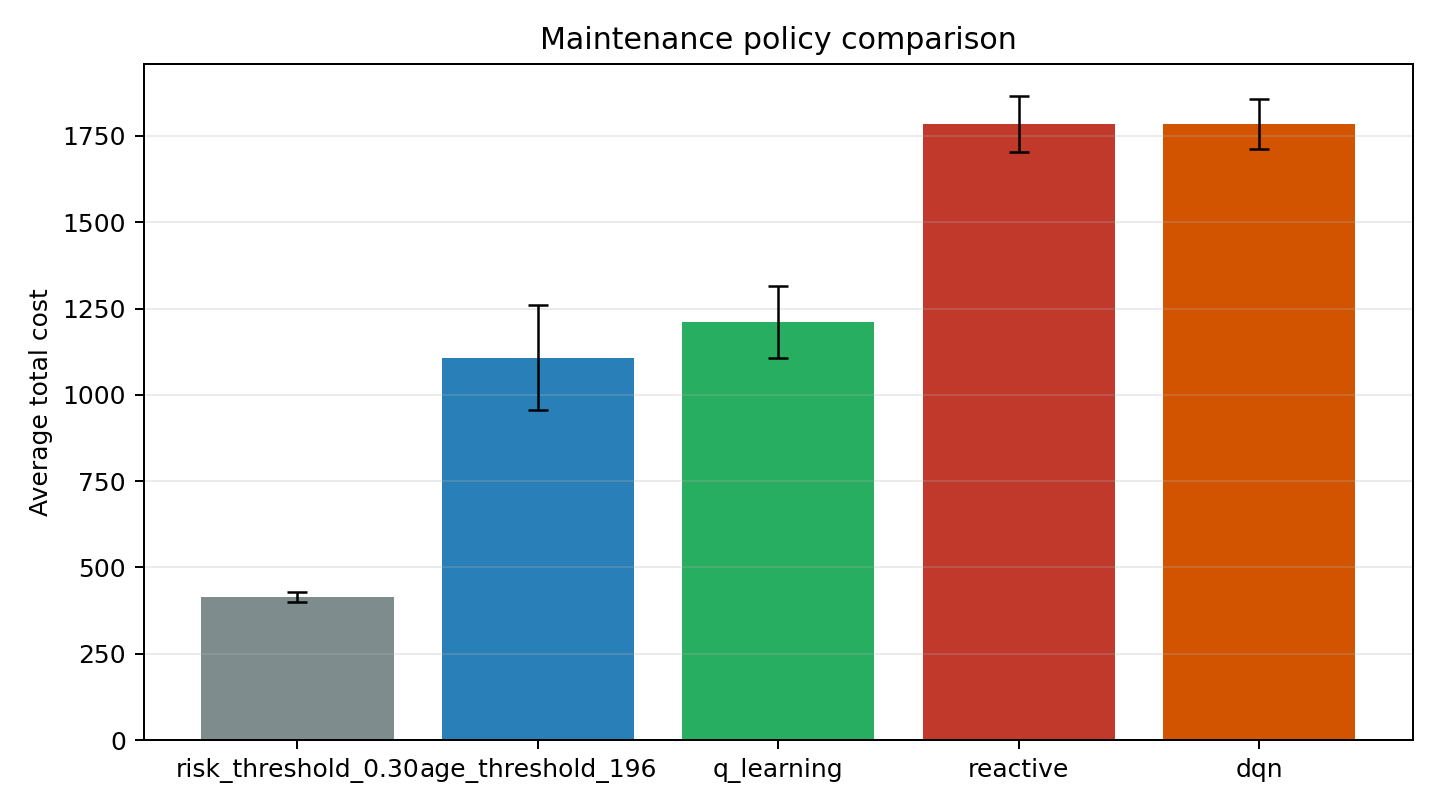
\includegraphics[width=0.72\textwidth]{../outputs/policy_comparison.png}
\caption{Average maintenance cost across competing policies.}
\label{fig:policy-comparison}
\end{figure}

\section{Discussion}
The strongest improvement in this project comes from better temporal representation rather than from a more complicated control algorithm. This is helpful for a course project because it keeps the main contribution easy to explain: rolling summaries, slopes, and lag structure turn noisy sensor streams into operationally useful risk estimates. The policy layer then demonstrates why that forecasting improvement matters.

\section{Limitations and Future Work}
The project uses synthetic data rather than a real industrial benchmark, and the RL layer is intentionally lightweight. Natural extensions include state-space or hidden Markov formulations, richer partially observed RL, and evaluation on datasets such as NASA C-MAPSS. The DQN baseline included in the repository is best treated as an extension rather than the main result.

\section{Reproducibility}
The full pipeline can be reproduced by installing the dependencies from \texttt{requirements.txt} and running \texttt{python run\_project.py}. The script regenerates all tables, figures, and both report formats. The notebook in \texttt{notebooks/final\_project\_analysis.ipynb} provides a complete end-to-end analysis starting from raw synthetic data generation.

\end{document}